\documentclass[dvipdfmx,autodetect-engine,titlepage]{jsarticle}
\usepackage[dvipdfm]{graphicx}
\usepackage{ascmac}
\usepackage{fancybox}
\usepackage{listings}
\usepackage{plistings}
\usepackage{itembkbx}
\usepackage{amsmath}
\usepackage{svg}
\usepackage{url}
\usepackage{graphics}
\usepackage{listings,jvlisting}
\usepackage{scalefnt}

\textheight=23cm
\renewcommand{\figurename}{図}
\renewcommand{\tablename}{表}
\newenvironment{code}
{\vspace{0.5zw}\VerbatimEnvironment  
\begin{screen} 
\baselineskip=1.0\normalbaselineskip
 \begin{Verbatim}}
{\end{Verbatim}
\baselineskip=\normalbaselineskip
 \end{screen}\vspace{0.5zw}} 

\title{情報理工学部 SNコース 2回\\
セキュリティ・ネットワーク学実験2\\
課題5-3レポート}
\author{2600200443-6\\Yamashita Kyohei\\山下 恭平}
\date{November 1 2021}

\begin{document}

\maketitle

\section{概要}
この実験では、Raspberry Piと超音波レンジャー、ブザーを用いて、物が接近した際に音で
警告するデバイスを設計した。このデバイスは、近年の自動車などによくみられる衝突回避
システムや、ストーブなどの安全装置の基礎となるデバイスだと考えた。

\section{外部仕様}

 \subsection{開発対象の使い方に関する説明}
  プログラム実行中、センサは超音波を用いて距離を測定し続ける。その距離が一定の値よりも
  小さい時、ブザーがなるように設計した。実際には、自分の手を近づけたり、遠ざけたりする
  ことで、距離を変化させ実験を行った。以下の図1は実際のデバイスの写真を撮ったものである。

 \begin{figure}[h]
  \centering
  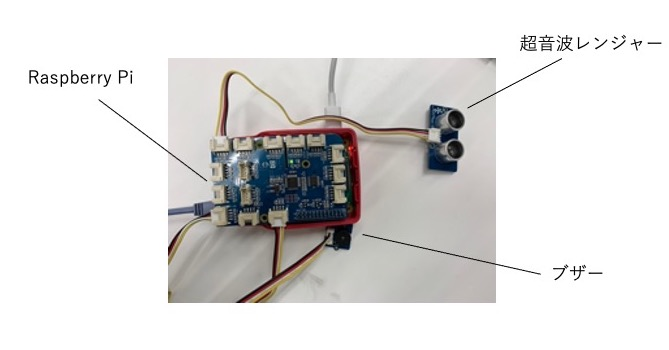
\includegraphics[scale=0.5]{pic1.jpg}
  \caption{開発したデバイス}
\end{figure}

 
 \subsection{開発対象を構成するハードウェアと、その主な仕様}
 Raspberry PiにはGrove Starter Kit のシールドを利用し、各センサやアクチュエータ
 を接続した。また、Raspberry Piはセンサから情報の取得、アクチュエータの制御など、デバイス
 の主要部分ほとんどを担っている。超音波レンジャーは超音波により距離を測定しており、精度は
 1cm単位で測定可能である。ブザーはRaspberry Piからの書き込み(0,1)によってon/offの切り替えが
 可能である。以下の表1はそれぞれのハードウェアを表にまとめたものである。

 \begin{table}[h]
  \centering
  \caption{ハードウェア一覧}
  \begin{tabular}{clll}
  \hline
  機器一覧            &  & \multicolumn{1}{c}{使用/情報}                  &  \\ \hline
  Raspberry Pi 4 Model B       &  & センサ、アクチュエータを接続し、取得した値の処理、条件分岐を行う。  &  \\ \hline
  超音波レンジャー      &  & 超音波を送り、物体からのエコーを受信し、距離を測定。 &  \\ \hline
  ブザー              &  & デジタル信号(0,1)でon/offが切り替え可能。                             &  \\ \hline
  \end{tabular}
  \end{table}
 
 \subsection{ハードウェアやソフトウェアが担当する機能と、機能同士の関連}
 超音波レンジャーは距離を測定し、ブザーは音を鳴らすという役割がある。\\
 この二つのハードウェアを制御しているのがRaspberry Piであある。Raspberry Pi上に
 書かれたプログラムは主に二つに分かれており。一つはセンサの値を取得する部分、もう一つ
 は、その値が一定の値よりも小さいかどうかを判別する部分である。また、判別する部分では
 、その判別結果に応じた出力をブザーに送っており、一定の値以下であれば1(ON)を、そうで
 なければ0(OFF)をブザーへ出力するようになっている。\\
 以下の図2は各機能の構成をまとめた図である。

 \begin{figure}[h]
  \centering
  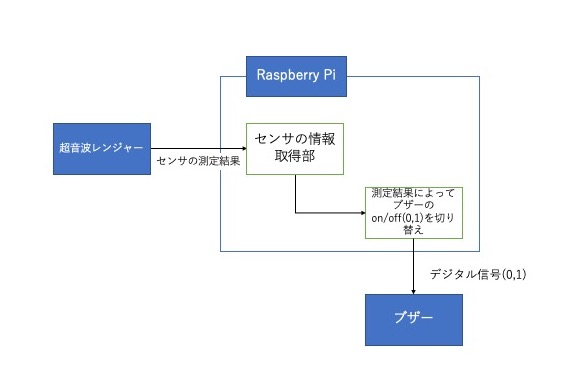
\includegraphics[scale=0.4]{pic2.jpg}
  \caption{機能構成図}
\end{figure}
 
 \subsection{開発に用いたプログラミング言語と開発環境}
 今回の実験では、 実際に各センサやアクチュエータを制御するためのプログラムを、「Ju
 pyter Notebook」で「Python」言語を用いて開発した。\\
 以下の表2は主な開発環境をまとめた表である。

 \begin{table}[h]
  \centering
  \caption{まとめ図}
  \begin{tabular}{clcl}
  \hline
  \multicolumn{4}{c}{主な開発環境}                          \\ \hline
  OS     &  & macOS Big Sur                        &  \\ \hline
  開発環境   &  & \multicolumn{1}{l}{Jupyter Notebook} &  \\ \hline
  使用した言語 &  & Python                               &  \\ \hline
  \end{tabular}
  \end{table}



\section{内部仕様}

  \subsection{各ハードウェアが備えるソフトウェアの詳細な設計}
  Raspberry Pi上のプログラムで、各センサ、アクチュエータを制御するための関数が
  用意されている、超音波レンジャーではultrasonicRead()という関数があり、測定した
  距離がint型で返ってくる。また、ブザーにおいては、digitalWrite()関数で(0,1)を書き込む
  ことで、ブザーのon/offを切り替えている。以下は、変数、関数をまとめた表である

  \begin{table}[h]
    \centering
    \caption{変数/関数 まとめ表}
    \begin{tabular}{ccll}
    \hline
                         & 変数名                                  & \multicolumn{1}{c}{説明}         &  \\ \hline
                         & ranger                               & 超音波センサのポート番号を指定するための変数。        &  \\ \hline
                         & buzzer                               & ブザーのポート番号を指定するための変数。           &  \\ \hline
                         & sensor\_value                        & センサから取得した値を格納する変数。             &  \\ \hline
    \multicolumn{1}{l}{} & \multicolumn{1}{l}{}                 &                                &  \\
                         &                                      & \multicolumn{1}{c}{}           &  \\ \hline
                         & 関数名                                  & \multicolumn{1}{c}{説明}         &  \\ \hline
    \multicolumn{1}{l}{} & \multicolumn{1}{l}{ultrasonicRead()} & 超音波センサが距離を測定するための関数。           &  \\ \hline
                         & digitalWrite()                       & ブザーへデジタル信号を書き込む関数。             &  \\ \hline
                         & pinMode()                            & 指定された入出力ポートに対して、入力か出力かを設定する関数。 &  \\ \hline
    \multicolumn{1}{l}{} & \multicolumn{1}{l}{}                 &                                & 
    \end{tabular}
    \end{table}

  \subsection{各ハードウェアが備えるソフトウェアにおける処理の流れ}
  このデバイスは、初めにセンサの値を取得し、その取得した結果を判定し、判定の結果
  に応じてブザーに信号を送る。といった流れを無限ループで回すことによって実現している。\\
  図3はその様子をフローチャートにまとめたものである。

  \begin{figure}[h]
    \centering
    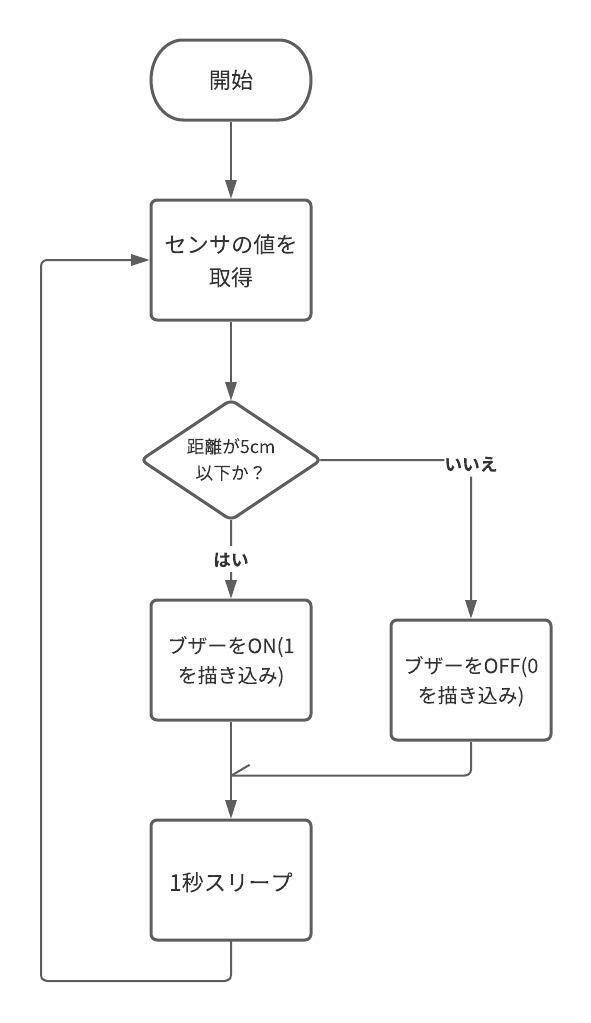
\includegraphics[scale=0.4]{pic3.jpeg}
    \caption{フローチャート}
\end{figure}

\section{実行例}
Jupyter Notebook上でプログラムを実行した後に、超音波レンジャーに手を
近づけてから、遠ざけるという一連の動作を行ったところ、手の距離が5cmあたりの
ところからブザーがなりはじめた。\\
図4は1秒おきのセンサの測定結果と、ブザーの状態をプリントしたJupyter Notebook上
のスクリーンショットであり。図5は実際に超音波レンジャーに手を近づける様子を写真に
撮ったものである。

\begin{figure}[h]
  \centering
  \begin{minipage}[b]{0.45\linewidth}
  \begin{center}
    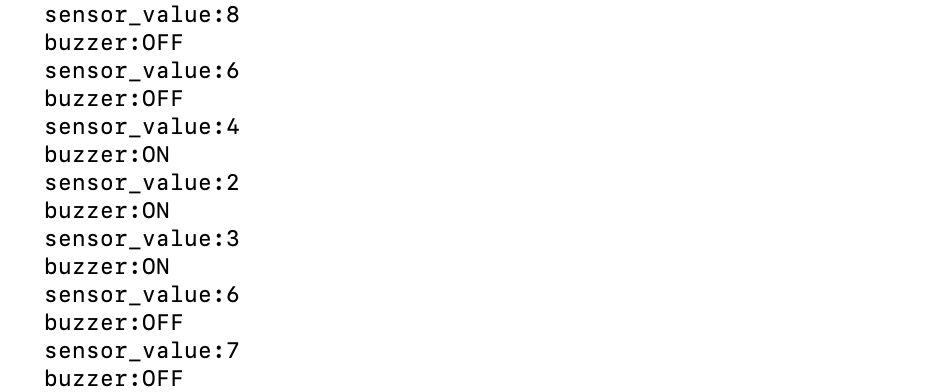
\includegraphics[keepaspectratio,scale=0.6]{pic4.png}
    \end{center}
    \caption{実行例1}
  \end{minipage}
  \begin{minipage}[b]{0.45\linewidth}
  \begin{center}
    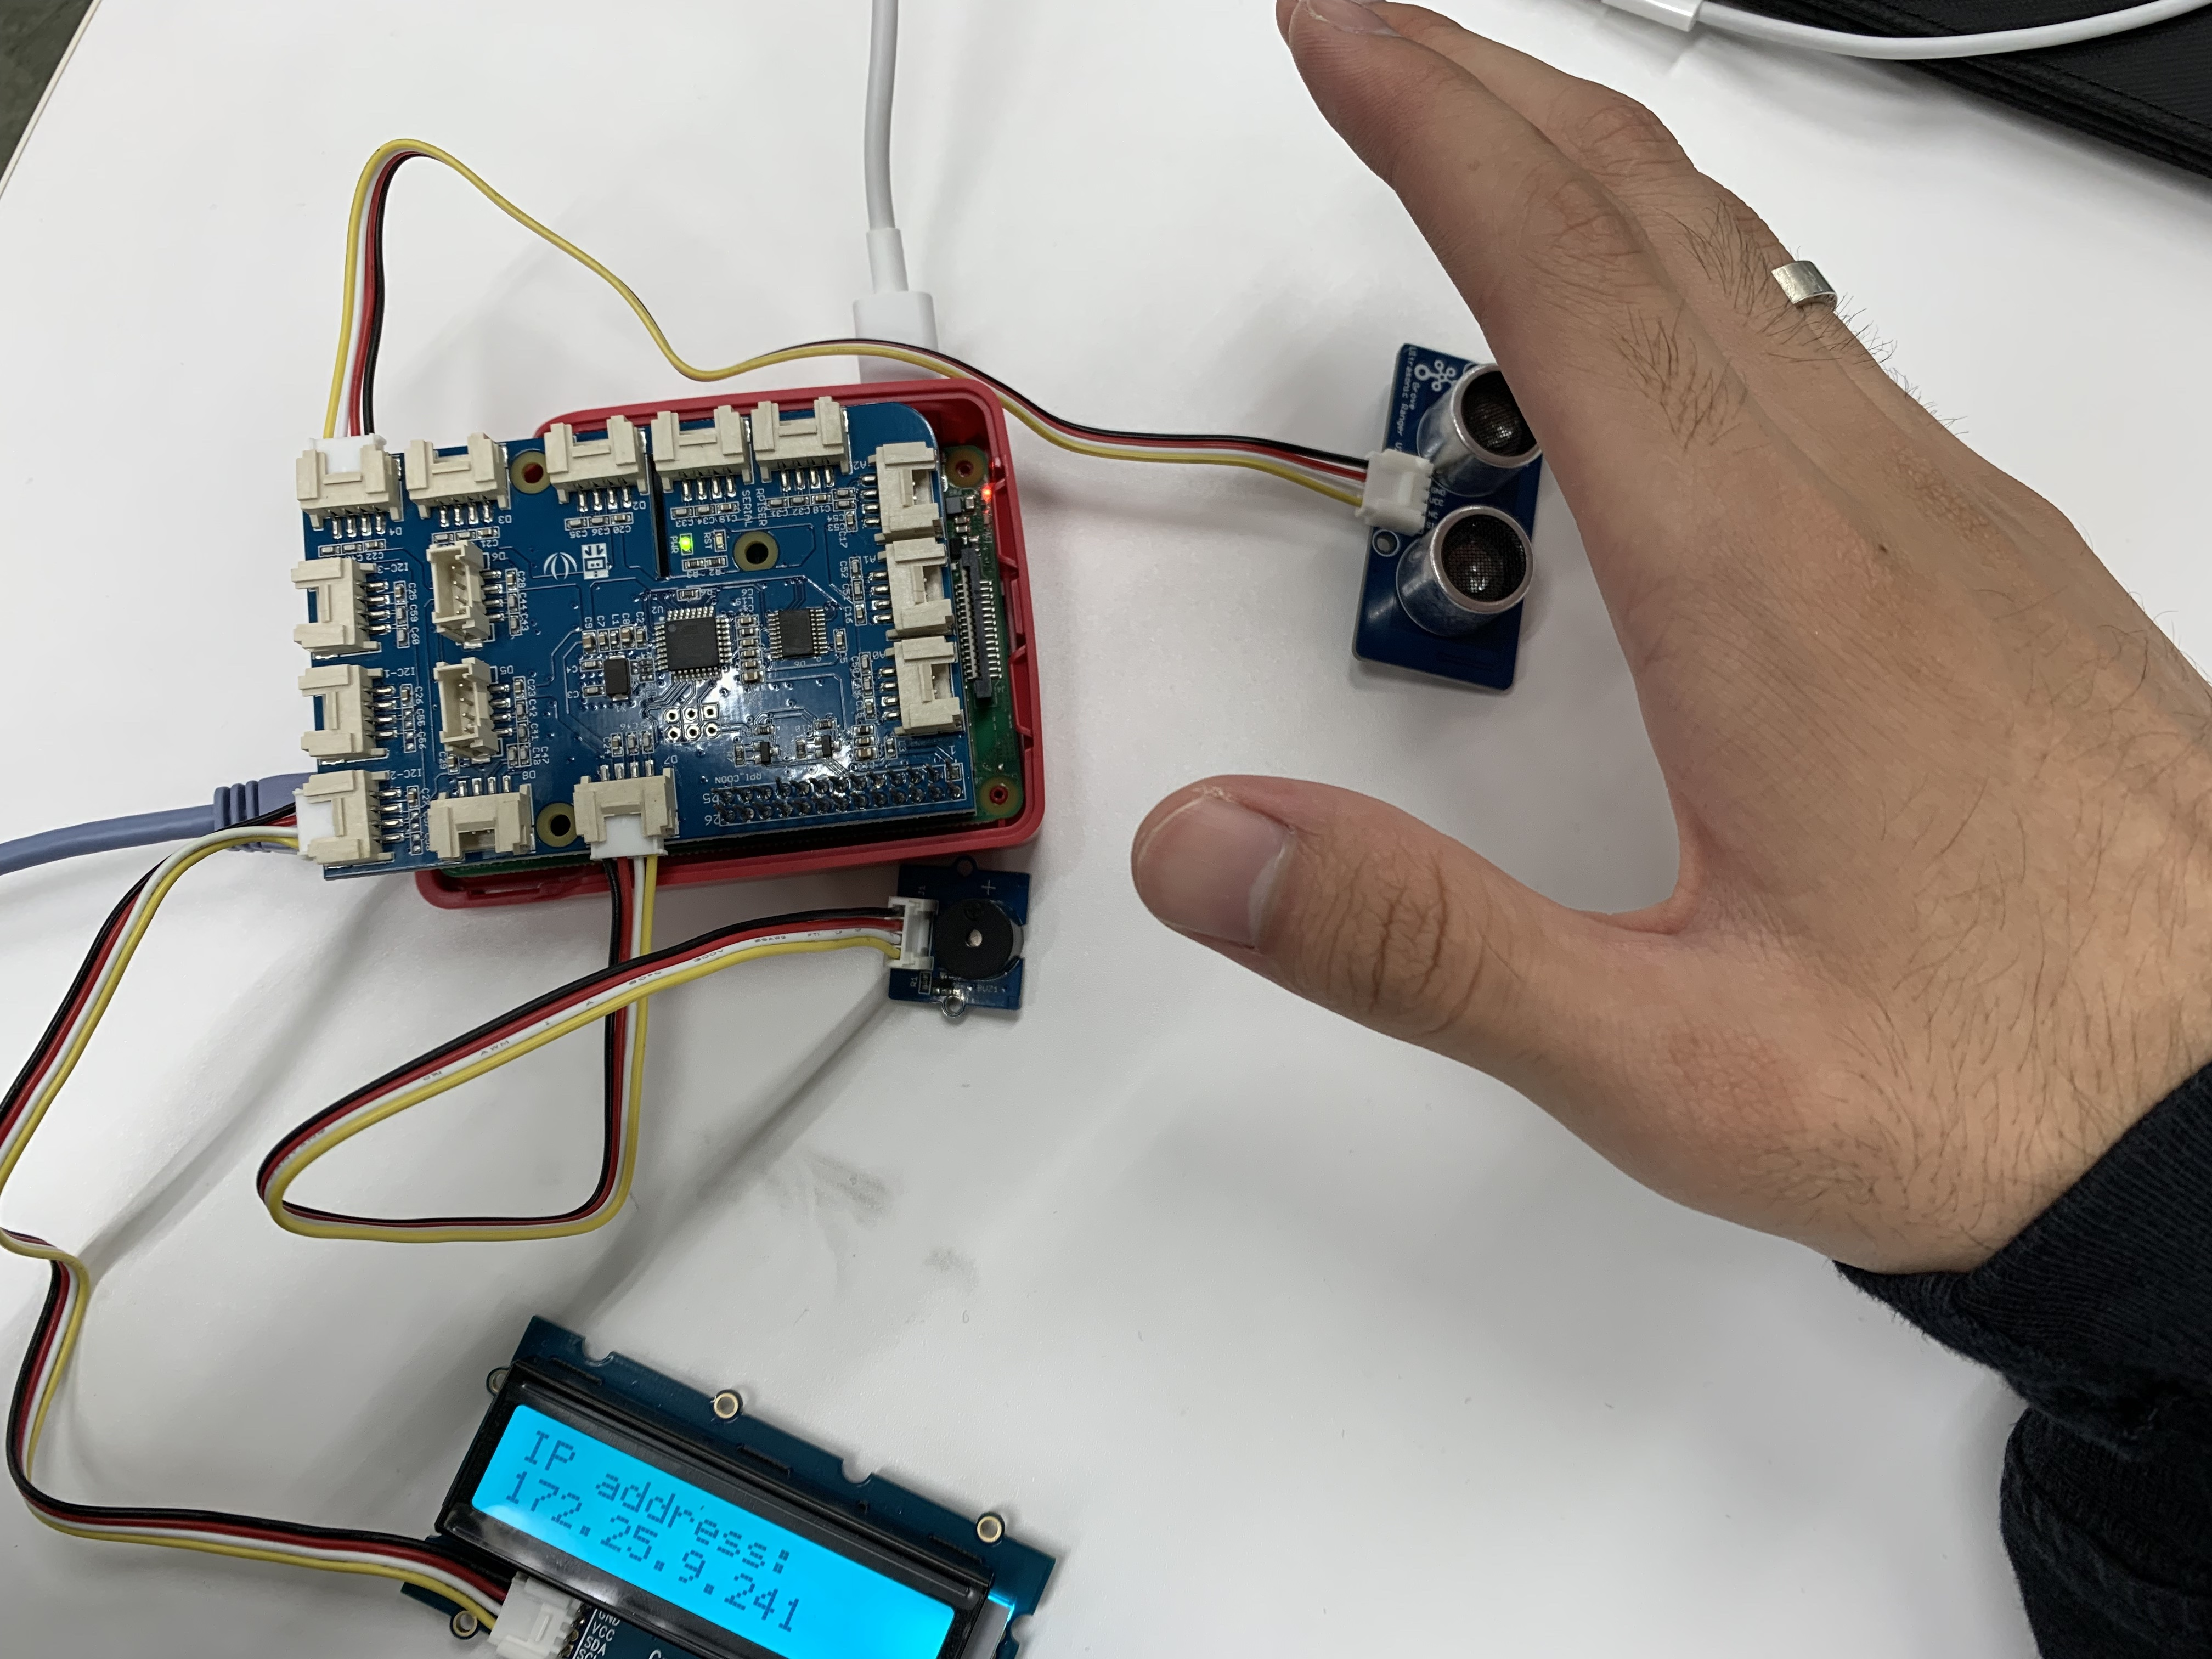
\includegraphics[keepaspectratio,scale=0.04]{pic5.jpg}
    \end{center}
    \caption{実行例2}
  \end{minipage}
\end{figure}


\section{ソースコード}
以下はソースコードである。\\
超音波レンジャーで測定した距離を20行目で取得し、取得した値を25行目から判別し、ブザー
のon/offを切り替えている。この全体の流れを16行目のwhile分で無限ループにしている。

  \lstset{
  basicstyle={\ttfamily},
  identifierstyle={\small},
  commentstyle={\smallitshape},
  keywordstyle={\small\bfseries},
  ndkeywordstyle={\small},
  stringstyle={\small\ttfamily},
  frame={tb},
  breaklines=true,
  columns=[l]{fullflexible},
  numbers=left,
  xrightmargin=0zw,
  xleftmargin=3zw,
  numberstyle={\scriptsize},
  stepnumber=1,
  numbersep=1zw,
  lineskip=-0.5ex
  }

  \begin{lstlisting}[caption=5-3.py,label=python]

    import time
    from grovepi import *
    
    # A4ポートへ超音波センサを接続
    ranger = 4
    
    # D5ポートへブザーを接続
    buzzer = 5
    
    # センサは入力、ブザーは出力として設定
    pinMode(ranger,"INPUT")
    pinMode(buzzer,"OUTPUT") 
    time.sleep(1)
    
    while True:
        try:
            
            # センサの値を読み込み
            sensor_value = ultrasonicRead(ranger)
            
            print("sensor_value:%d" %(sensor_value))
            
            # 5以下ならブザーON
            if sensor_value < 5:
                print("buzzer:ON")
                digitalWrite(buzzer,1)
            else:
                print("buzzer:OFF")
                digitalWrite(buzzer,0)
            
            time.sleep(1)
                
        except KeyboardInterrupt:
            break
            
        except IOError:
            print ("Error")


  \end{lstlisting}


\end{document}

